\chapter{Erstellung von Orthofotos der HSR}

%----------------------------------------------------------------------------------------

Die folgenden Kapitel beschreiben den Prozess, der nötig war um ein Orthofoto
sowie ein georeferenziertes texturiertes Oberflächenmodell der Hochschule für
Technik in Rapperswil zu erzeugen.

%----------------------------------------------------------------------------------------

\section{Erfassung des HSR-Geländes mit Kamera-Drohne}

Auf die Erfassung von Luftbildern mithilfe eines Multikopters sind wir bereits
in \autoref{workflow:drone} eingegangen. Deshalb möchten wir hier lediglich die
Unterschiede zur 3D-Erfassung des Schloss Rapperswils hervorheben.

Im Gegensatz zur 3D-Erfassung geht es bei der Herstellung von Orthofotos nicht
primär um die dreidimensionale Form eines Objektes, sondern darum, möglichst
senkrechte und verzerrungsfreie Bilder zu erstellen.

\needspace{8\baselineskip}
Wir haben wiederum den Team BlackSheep Discovery Pro Quadrokopter mit Gimbal
verwendet, diesmal jedoch nicht mit der GoPro Kamera, sondern mit einer Sony
Alpha 5100 und einer verzerrungsfreien Brennweite.
\begin{figure}[H]
	\centering
	\includegraphics[width=\textwidth]{images/copter1.jpg}
	\caption{Der Team BlackSheep Discovery Pro Quadrokopter}
	\label{img:copter1}
\end{figure}

\needspace{8\baselineskip}
\noindent Die Kamera wurde mit dem Gimbal so positioniert, dass sie senkrecht
nach unten zeigt.
\begin{figure}[H]
	\centering
	\includegraphics[width=\textwidth]{images/copter3.jpg}
	\caption{Die Kamera-Aufhängung}
	\label{img:copter3}
\end{figure}

\needspace{8\baselineskip}
\noindent Während wir beim ersten Versuch ein Smartphone als GPS-Tracker auf dem
Quadrokopter befestigt hatten, verwendeten wir diesmal ein dediziertes
GPS-Tracking-Gerät, ein \textit{Navin
miniHomer}\footnote{\url{https://www.znex.de/de/minihomer/}}. Der Tracker wurde
so konfiguriert, dass er 10 mal pro Sekunde die Position und Ausrichtung
aufzeichnete.
\begin{figure}[H]
	\centering
	\includegraphics[width=\textwidth]{images/copter2.jpg}
	\caption{Deutlich sichtbar: Der gelbe GPS-Tracker}
	\label{img:copter2}
\end{figure}

\needspace{8\baselineskip}
\noindent Während 10 Minuten flogen wir nun auf einer Höhe zwischen 50m und 120m
über das HSR-Gelände, um Bildmaterial von jedem Gebäude zu erhalten.
\begin{figure}[H]
	\centering
	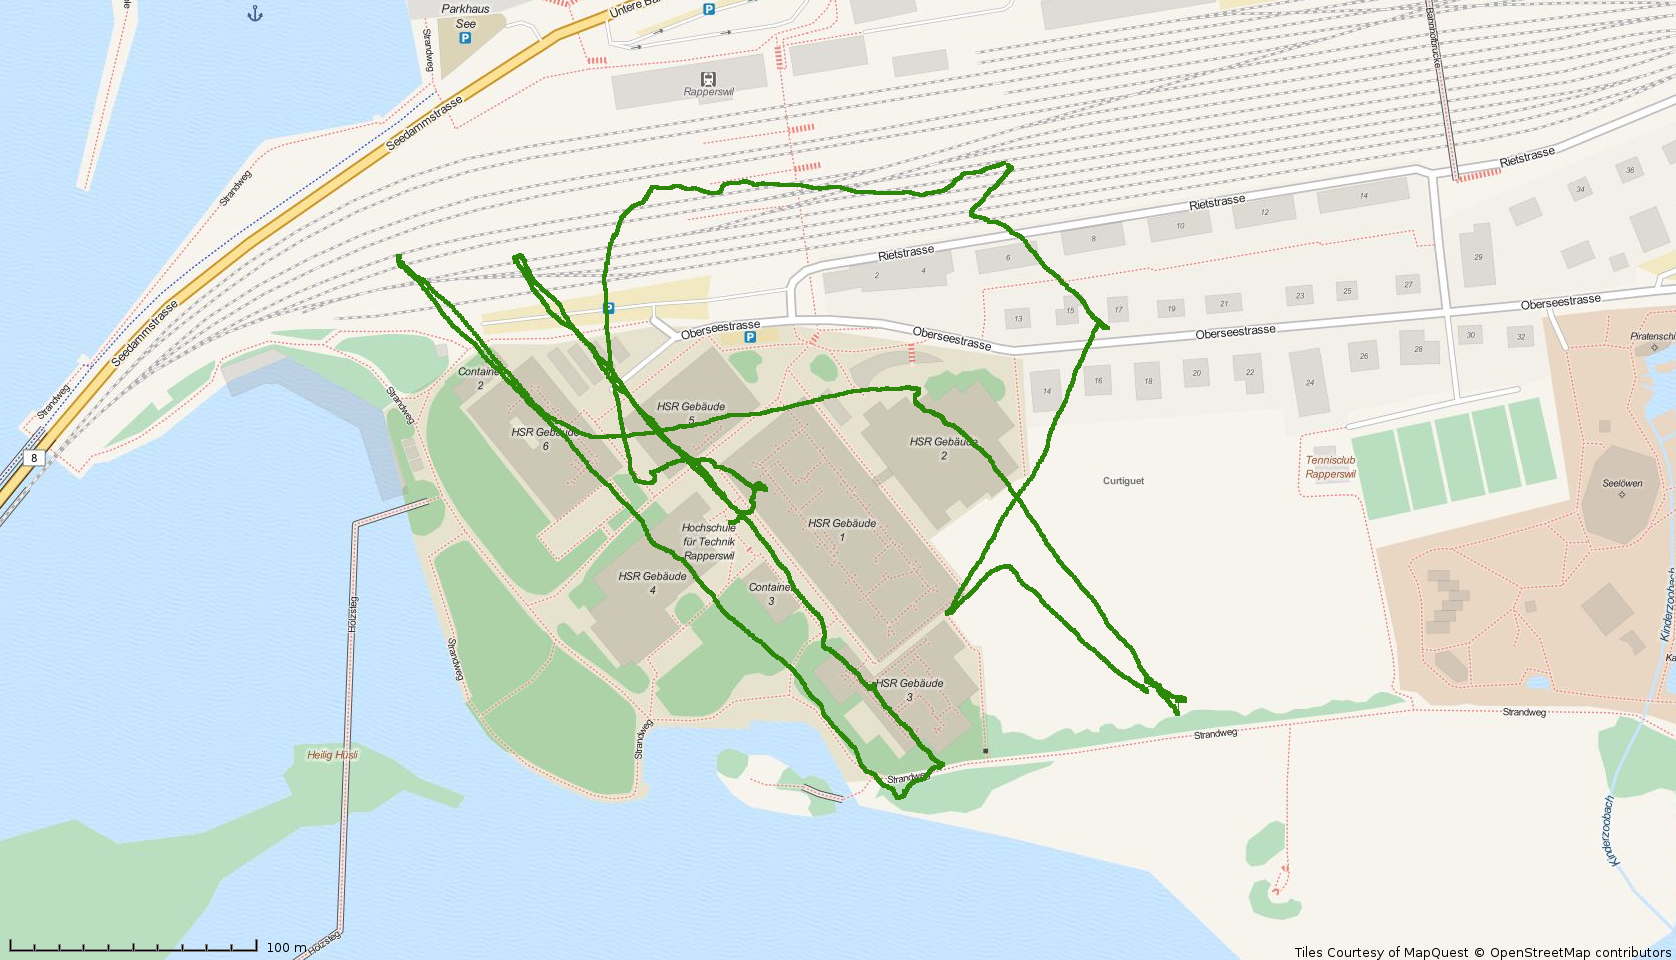
\includegraphics[width=\textwidth]{images/gpstrace_hsr_mapquest}
	\caption{GPS Trace des Quadkopters während der Erfassung.}
	\label{img:gpstrace_hsr_mapquest}
\end{figure}

%----------------------------------------------------------------------------------------

\section{Geocoding der Bilder}

\label{workflow:hsr:geocoding}

Zurück zuhause sortierten wir die Bilder und löschten unbrauchbares
Bildmaterial. Anschliessend exportierten wir den GPS-Trace mithilfe von
\textit{GPSBabel}\footnote{\url{http://www.gpsbabel.org/}}:

\vspace{0.5\baselineskip}
\begin{minted}[bgcolor=tango-bg,frame=lines,framesep=2mm,samepage=true,fontsize=\footnotesize]{bash} 
gpsbabel -i skytraq -f /dev/ttyUSB0 -o gpx -F gps-recording.gpx
\end{minted}

Anschliessend muss diese Information in die Bild-Metadaten geschrieben werden.
Den Aufnahmezeitpunkt der Fotos kann mit dem Speicherzeitpunkt der
GPS-Messpunkte korreliert werden um so die entsprechende Position zu finden.

Um dies zu bewerkstelligen, gibt es verschiedene Tools. Wir haben
\textit{GPicSync}\footnote{\url{https://code.google.com/p/gpicsync/}} verwendet,
um die Geodaten im
IPTC-Format\footnote{\url{https://de.wikipedia.org/wiki/IPTC-IIM-Standard}} in
den Bildern zu speichern. Die verwendeten Einstellungen sind in
\autoref{img:gpicsync} ersichtlich.

\begin{figure}[h!]
	\centering
	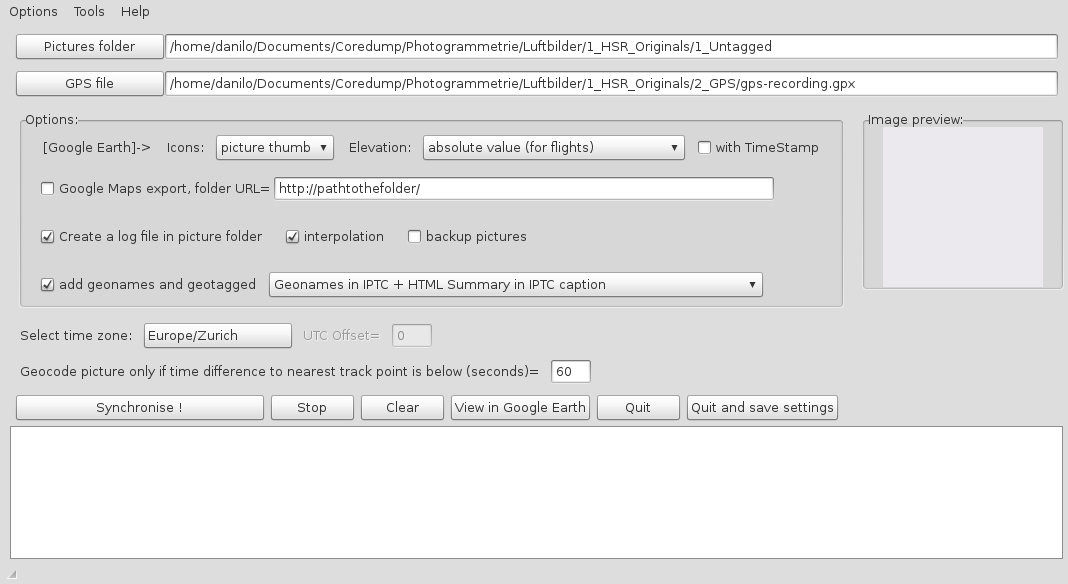
\includegraphics[width=\textwidth]{images/gpicsync}
	\caption{Einstellungen GPicSync}
	\label{img:gpicsync}
\end{figure}

Wichtig ist dabei vor allem ein möglicher Offset zwischen Kamera-Uhrzeit und
GPS-Uhrzeit. Man kann diese Abweichung relativ einfach berechnen, indem man ein
Foto des GPS-Geräts erstellt, auf welchem die genaue Uhrzeit ablesbar ist.
Der Offset ist die Differenz zwischen der Uhrzeit auf dem Foto und der Uhrzeit
in den Bild-Metadaten.

In \textit{GPicSync} kann der Offset über \texttt{Options > Local time
correction} konfiguriert werden, indem man die Uhrzeit beider Geräte eintippt.

%----------------------------------------------------------------------------------------

\section{Einführung OpenDroneMap}

OpenDroneMap (\url{https://github.com/OpenDroneMap/OpenDroneMap}) ist ein
Projekt, welches im Jahr 2014 von Stephen Mather ins Leben gerufen
wurde\cite{smathermather:2014}. Es beinhaltet eine Sammlung von Scripts, um
Bilder von Multikoptern, Heissluftballonen, Drachen oder anderen Luftfahrzeugen
in diverse Formate zu konvertieren.

Der aktuelle Funktionsumfang beinhaltet als Zielformate Punktwolken,
Oberflächenmodelle, Texturierte Oberflächenmodelle und Orthofotos. Zudem kann
OpenDroneMap auch Geodaten aus den EXIF- oder IPTC-Daten der Bilder verwenden.
Alternativ kann auch eine Datei mit Vollpasspunkten (Englisch: Ground Control
Points) bereitgestellt werden, welche für die georeferenzierung verwendet wird.

Um dies zu erreichen, integriert OpenDroneMap viele existierende Open Source
Libraries wie CMVS, PMVS, Graculus und weitere. Es gibt also eine deutliche
Überschneidung mit der in VisualSFM verwendeten Toolchain aus
\autoref{workflow:vsfm}.

Anders als VisualSFM ist OpenDroneMap jedoch kein GUI\-/Programm, sondern wird
rein auf der Kommandozeile ausgeführt. Viele Parameter ermöglichen die Anpassung
und Optimierung des Prozesses.

Das Bemerkenswerte an OpenDroneMap ist, dass es die erste Open Source Toolchain
seiner Art ist. Bisher gab es keinerlei freie Software, die die ganze
Photogrammetrie-Pipeline von den Fotos bis zum Orthofoto und Oberflächenmodell
abgedeckt haben. Kommerzielle Alternativen dazu sind teure Programme wie Pix4D
oder Agisoft PhotoScan.

OpenDroneMap hat eine aktive Community, seit 2014 haben bereits 30 verschiedene
Personen Code dazu beigesteuert. Es lohnt sich, die Entwicklung des Projektes
weiter zu verfolgen.

%----------------------------------------------------------------------------------------

\section{Installation OpenDroneMap}

\subsection{Lokale Installation}

OpenDroneMap setzt eine Ubuntu 12.04 oder 14.04 Installation voraus. Das
Projekt liefert ein Installations-Script mit, welches alle benötigten
Abhängigkeiten installiert und dann die mitgelieferten Komponenten kompiliert.

\vspace{0.5\baselineskip}
\begin{minted}[bgcolor=tango-bg,frame=lines,framesep=2mm,samepage=true,fontsize=\footnotesize]{bash} 
git clone https://github.com/OpenDroneMap/OpenDroneMap
cd OpenDroneMap
./install.sh
\end{minted}

\noindent Nun kann das Haupt-Script von einem Bilder-Ordner aus aufgerufen werden.

\vspace{0.5\baselineskip}
\begin{minted}[bgcolor=tango-bg,frame=lines,framesep=2mm,samepage=true,fontsize=\footnotesize]{bash} 
cd /path/to/images
/path/to/opendronemap/run.pl
\end{minted}

\noindent Der Nachteil dieser Methode liegt darin, dass man dem Script vertrauen
muss, dass es keine "<Unordnung"> hinterlässt. Es gibt keinen Uninstaller.

\subsection{Vagrant / VirtualBox}

Auf \url{https://github.com/OpenDroneMap/odm_vagrant} findet sich eine
Anleitung, wie man mithilfe von
Vagrant\footnote{\url{https://www.vagrantup.com/}} eine
VirtualBox\footnote{\url{https://www.virtualbox.org/}} VM starten und
initialisieren kann, welche dann OpenDroneMap ausführt.

Der Vorteil davon ist die Isolation des Systemes - wenn man die Software nicht
mehr benötigt kann man einfach die VM löschen. Zudem läuft die Virtuelle
Maschine auch auf Systemen die OpenDroneMap nicht unterstützen, wie Windows oder
OS X. Nachteile ist vor Allem der grosse Overhead der Virtualisierung.

\subsection{Docker}

Das beste aus zwei Welten bietet Docker\footnote{\url{https://www.docker.com/}},
eine Software für die Erstellung und den Betrieb von Linux-Containern auf Basis
von LXC oder libcontainer. Dabei wird nicht die ganze Hardware virtualisiert,
sondern lediglich das Betriebssystem. Der Kernel hingegen wird mit dem
Host-System geteilt. Um dies zu erreichen, werden Linux Kernel-Features wie
Control Groups und Kernel Namespaces verwendet.

Diese Lösung erlaubt die Isolation einer Applikation, hat aber einen extrem
geringen Overhead. Der Container startet innerhalb von Millisekunden, nicht
innerhalb von Minuten wie bei VirtualBox.

OpenDroneMap verfügt bisher über kein offizielles Docker\-/Image, wir haben
jedoch das dafür benötigte Dockerfile geschrieben und dem Projekt einen Pull
Request
gesendet\footnote{\url{https://github.com/OpenDroneMap/OpenDroneMap/pull/143}}.
Inzwischen wurde der Pull Request gemerged, daher kann diese Deployment-Methode
nun sehr einfach getestet werden:

\vspace{0.5\baselineskip}
\begin{minted}[bgcolor=tango-bg,frame=lines,framesep=2mm,samepage=true,fontsize=\footnotesize]{bash} 
git clone -b docker https://github.com/OpenDroneMap/OpenDroneMap
cd OpenDroneMap
export IMAGES=/absolute/path/to/your/images
docker build -t opendronemap:latest .
docker run -v $IMAGES:/images opendronemap:latest
\end{minted}

Docker läuft nativ nur unter Linux. Für Windows und OS X Systeme gibt es jedoch
mit Boot2Docker eine einfache Möglichkeit, Docker trotzdem zu nutzen:

\begin{itemize}
	\item \url{https://docs.docker.com/docker/installation/windows/}
	\item \url{https://docs.docker.com/docker/installation/mac/}
\end{itemize}

%----------------------------------------------------------------------------------------

\section{Generierung Orthofoto und Oberflächenmodell}

\label{workflow:hsr:generate}

Wie im letzten Kapitel bereits gezeigt, wird OpenDroneMap mithilfe des
\texttt{run.pl} Scripts aus dem Bilder-Ordner heraus gestartet.

Zuerst muss man also einen Ordner mit allen Bildern vorbereiten. Wir haben ein
geeignetes Subset der zuvor in \autoref{workflow:hsr:geocoding} geocodierten
Bilder (124 Stück) ausgewählt und in einen separaten Ordner kopiert.

Sehr wichtig ist, dass die Bilder über eine klein geschriebene Dateiendung
verfügen. Aufgrund eines Bugs in
OpenDroneMap\footnote{\url{https://github.com/OpenDroneMap/OpenDroneMap/issues/33}}
können die Bilder ansonsten aktuell nicht verarbeitet werden. Falls die Bilder
aktuell noch über eine gross geschriebene Endung verfügen, könenn sie mit
folgendem Befehl einfach umbenannt werden:

\vspace{0.5\baselineskip}
\begin{minted}[bgcolor=tango-bg,frame=lines,framesep=2mm,samepage=true,fontsize=\footnotesize]{bash} 
for file in *.JPG; do mv "$file" "`basename $file .JPG`.jpg"; done
\end{minted}

Anschliessend kann OpenDroneMap gestartet werden. Da wir keine Ground Control
Points bereitstellen, muss noch eine entsprechende Operation mitgegeben werden.

\vspace{0.5\baselineskip}
\begin{minted}[bgcolor=tango-bg,frame=lines,framesep=2mm,samepage=true,fontsize=\footnotesize]{bash} 
# Normale Installation
/path/to/opendronemap/run.pl --odm_georeferencing-useGcp false

# Docker
docker run --rm -v $(pwd):/images opendronemap:latest \
       --odm_georeferencing-useGcp false
\end{minted}

\noindent Der Prozess dauerte bei unserem Datensatz knapp 3 Stunden.

%----------------------------------------------------------------------------------------

\section{Resultate}

Die Resultate der Verarbeitung befinden sich in einem Unterordner des
Bildverzeichnisses mit dem Namen
\texttt{reconstruction\-/with\-/image\-/size\-/2400\-/results}.

\subsection{Orthofoto}

Das Orthofoto hat den Namen \texttt{odm\_orthophoto.png}. In unserem Fall war es
14'236 $\times$ 14'143 Pixel (ca. 200 Megapixel) und 120 MiB gross.

\begin{figure}[H]
	\centering
	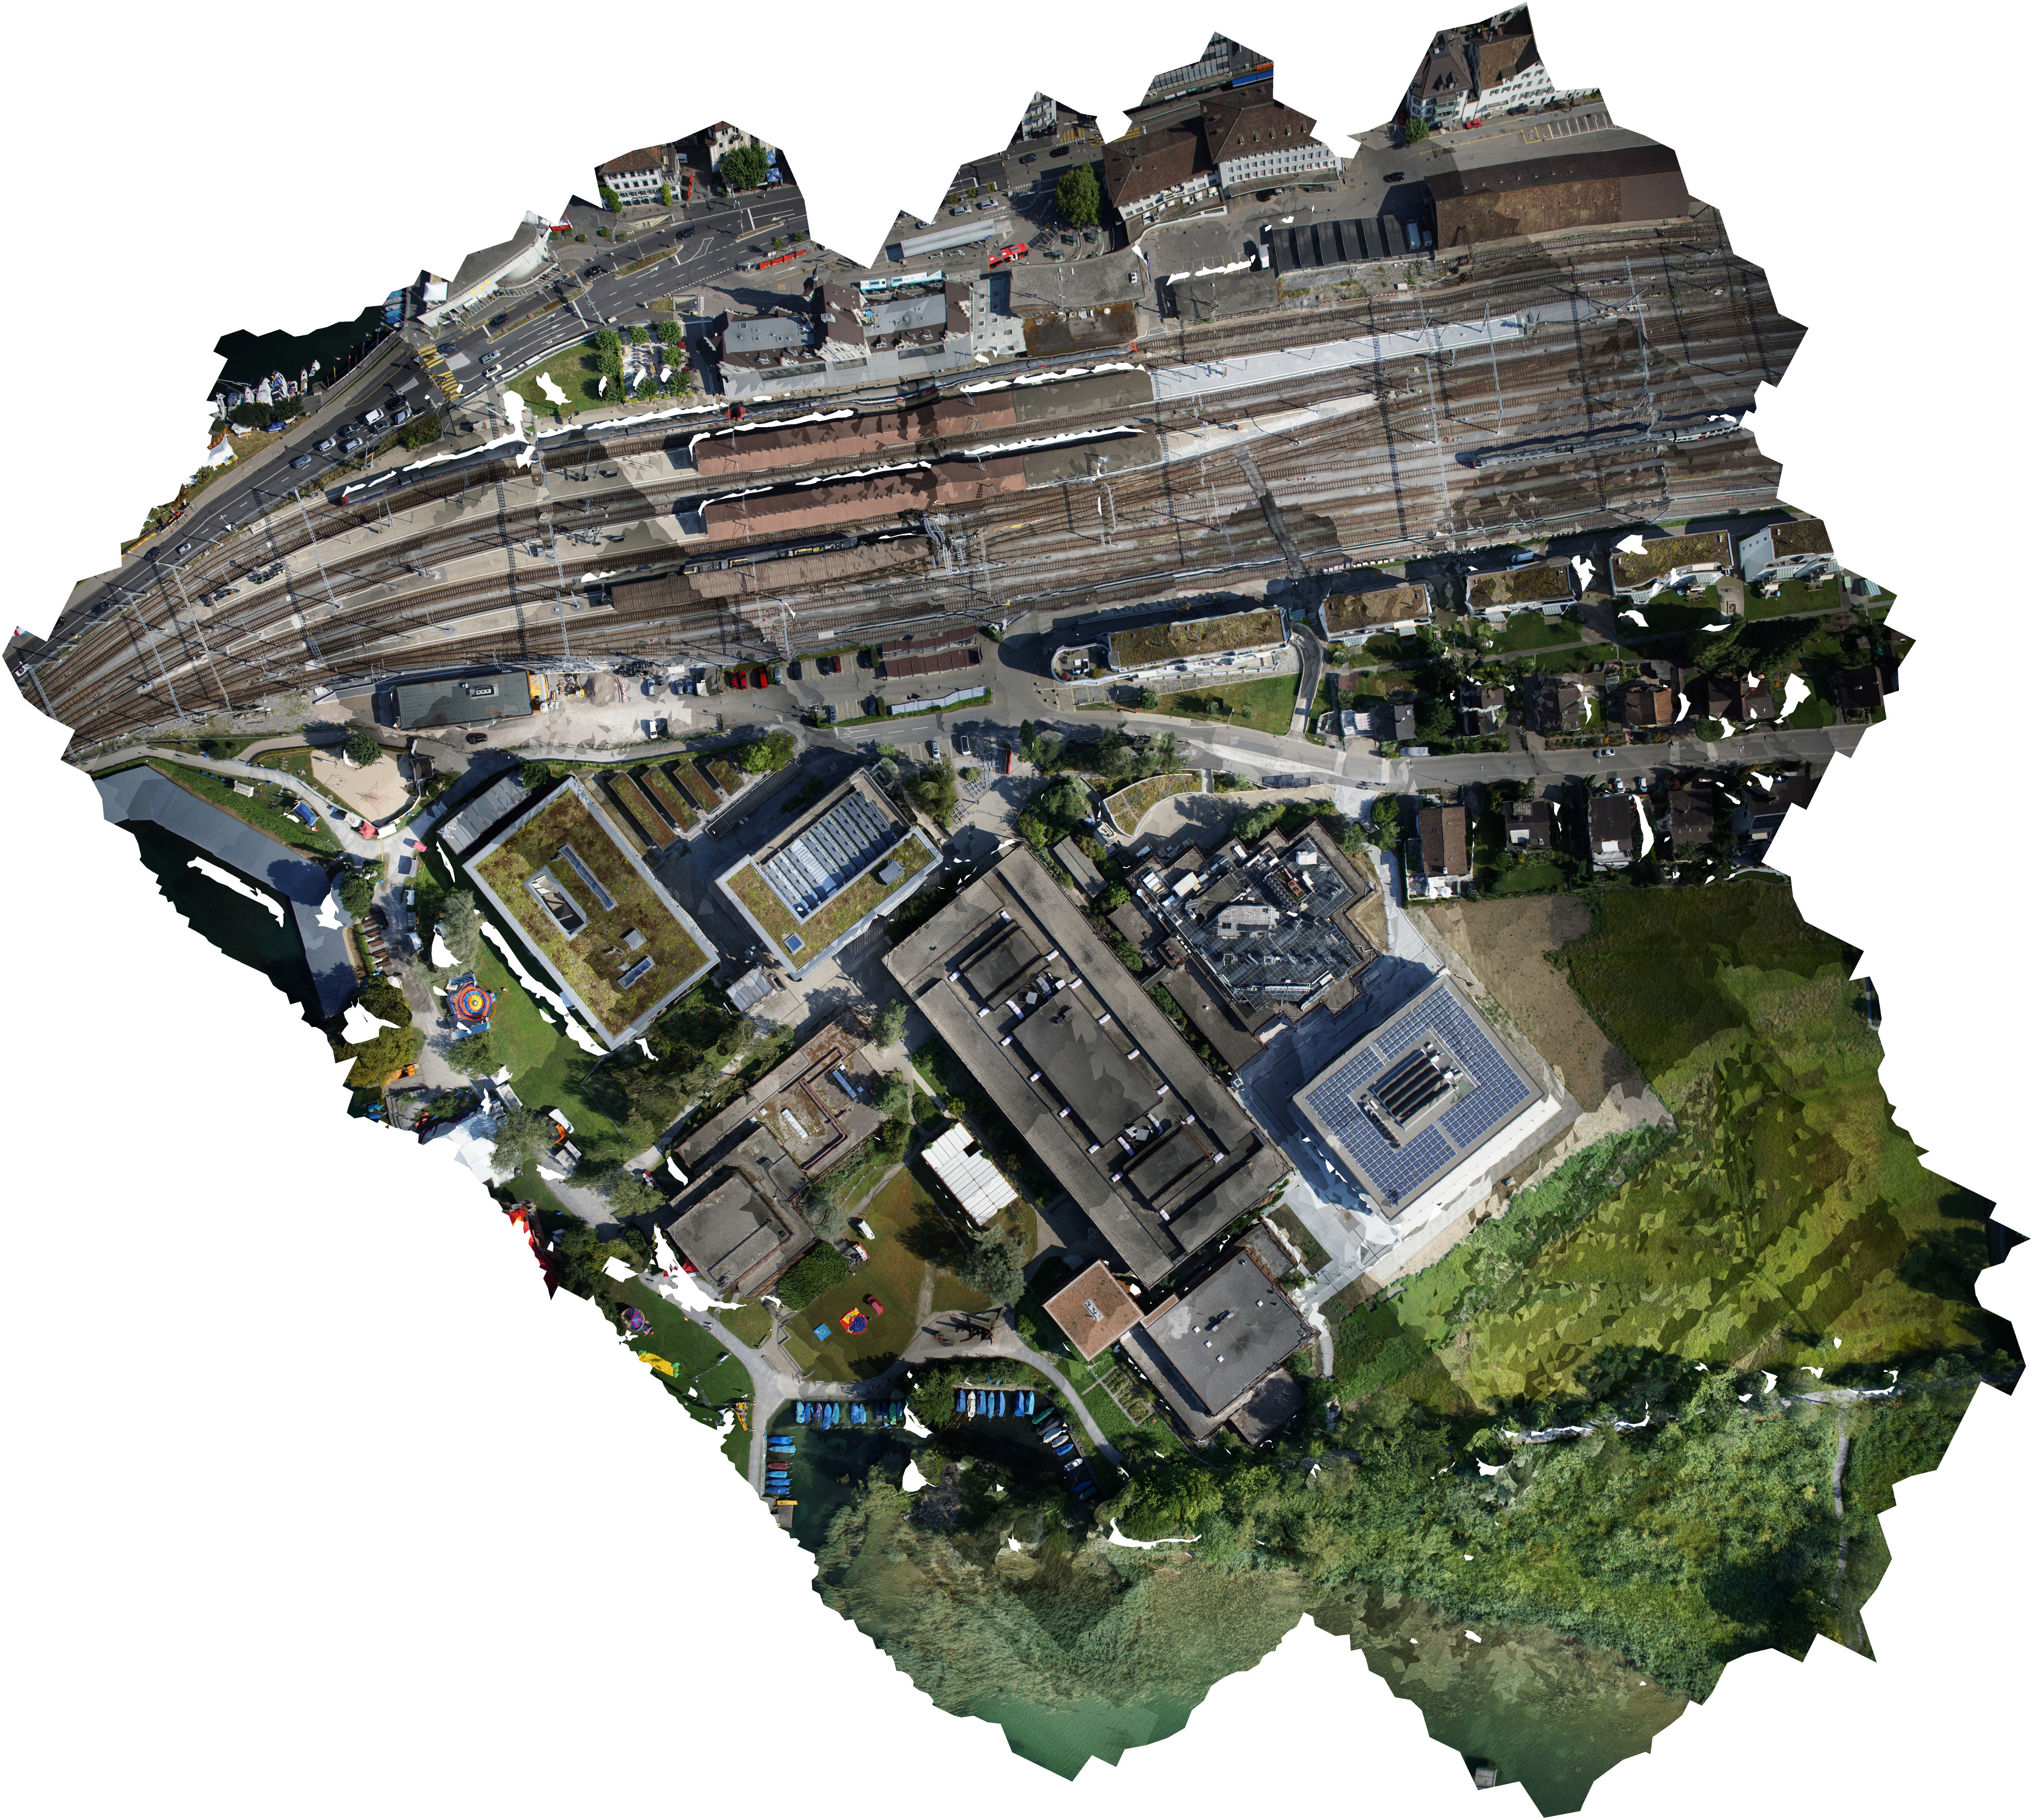
\includegraphics[width=\textwidth]{images/odm_orthophoto}
	\caption{Resultierendes Orthofoto des HSR-Areals}
	\label{img:odm_orthophoto}
\end{figure}

\noindent Wie man sieht, ist das Luftbild orthorektifiziert, d.h. die Rotation
stimmt mit den effekiven Himmelsrichtungen überein. Dies ist dank den
eingebetteten GPS-Metadaten möglich.

\subsection{Texturiertes Oberflächenmodell}

OpenDroneMap erzeugt nicht nur ein 2D-Luftbild, sondern auch ein
orthorektifiziertes und texturiertes 2.5D-Oberflächenmodell. Dieses befindet
sich im Unterordner \texttt{odm\_texturing}. Das Modell
(\texttt{odm\_tex\-tu\-ring/\-odm\_textured\_model\_geo.obj}) kann
beispielsweise mit MeshLab geöffnet werden.

\begin{figure}[H]
	\centering
	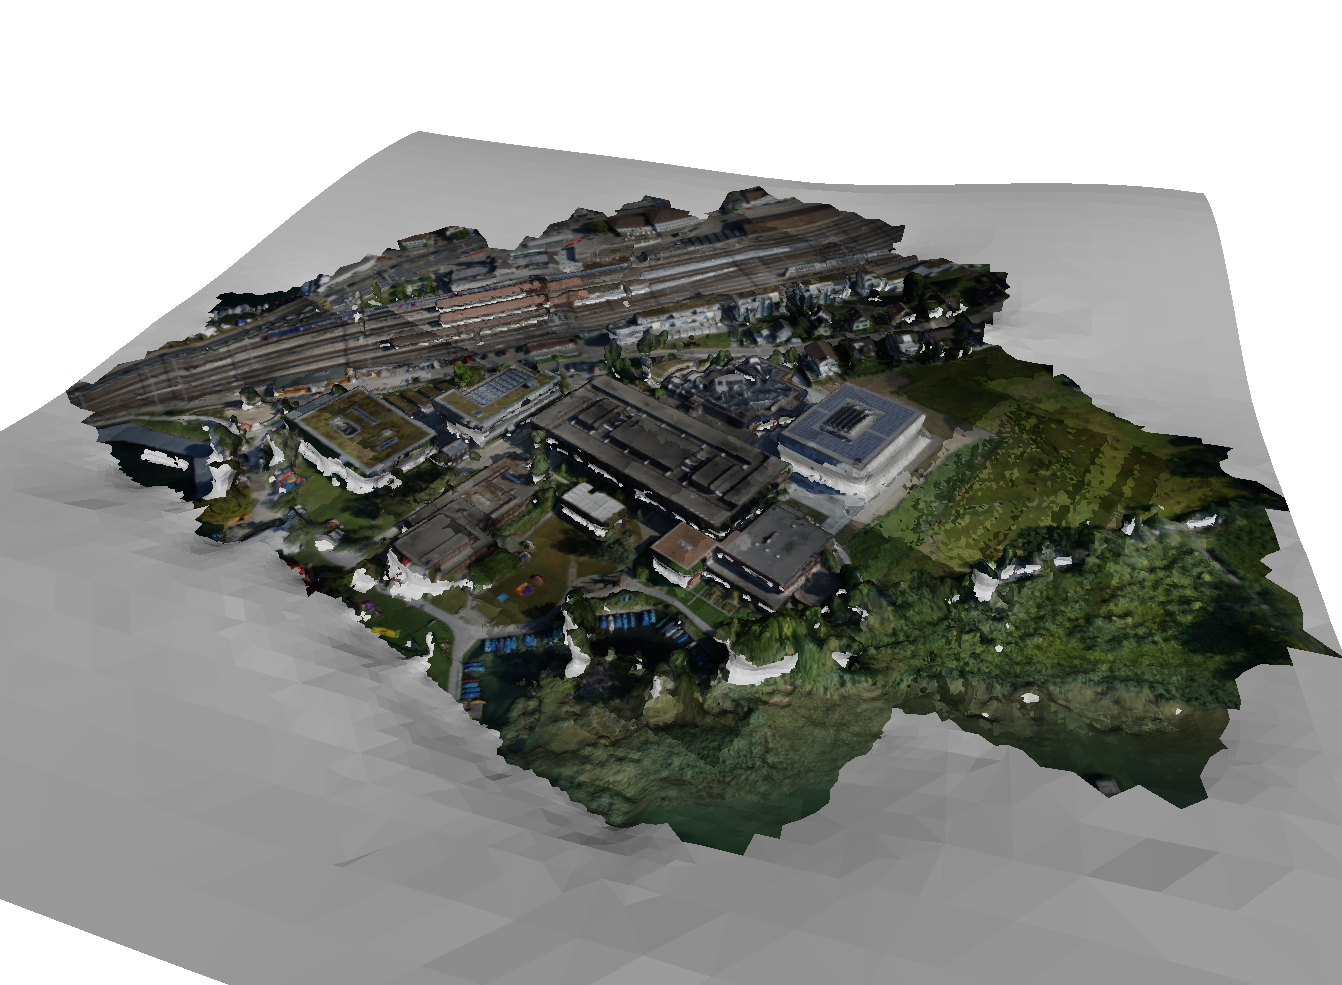
\includegraphics[width=\textwidth]{images/odm_mesh}
	\caption{Resultierendes Oberflächemodell des HSR-Areals}
	\label{img:odm_mesh}
\end{figure}

\noindent Das untexturierte Mesh kann online unter
\url{https://sketchfab.com/models/3dd7e0e053054e06b526d2c478253cef} betrachtet
werden.

\subsection{Beurteilung der Resultate}

Dafür, dass wir OpenDroneMap in der Standardkonfiguration ohne weitere
Anpassungen über die Bilder haben laufen lassen, sehen die Resultate sehr
beeindruckend aus. Rückwirkend gäbe es ein paar Dinge, die wir verbessern
würden:

\begin{itemize}
	\item Das Orthofoto weist immer noch Lücken auf. Bei einem zweiten Versuch
		würden wir mehr Bildmaterial sammeln.
	\item Wir haben rein senkrechte Bilder erstellt. Das reicht zwar für das
		Orthofoto aus, im texturierten Oberflächenmodell sieht man jedoch viele
		weisse, unförmige Wände. Dies würde sich durch eine 45$^{\circ}$-Erfassung des
		Geländes wohl stark verbessern.
	\item Das Orthofoto ist nicht georeferenziert, sondern lediglich
		orthorektifiziert: Die Himmelsrichtungen stimmen mit der Ausrichtung des
		Bildes überein. Für eine korrekte Georeferenzierung müsste man OpenDroneMap
		eine Liste von Ground Control Points übergeben (siehe
		\autoref{workflow:hsr:generate}). Dies wird voraussichtlich in einer
		zukünftigen Version von OpenDroneMap behoben. Alternativ kann man das Bild
		mit einem Tool wie QGIS\footnote{\url{http://qgis.org/}} georeferenzieren.
\end{itemize}

%----------------------------------------------------------------------------------------

\section{Weitere Ressourcen}

Hier listen wir ein paar weitere Ressourcen auf, die wir während unserer Arbeit
gefunden haben.

\subsection{Mapknitter}

Auf \url{http://mapknitter.org/} existiert ein Projekt zur einfachen Erstellung
von Luftbildern (aerial maps). Der Workflow ist jedoch manuell, d.h. die
Luftbilder werden auf eine Karte gezogen und dort "<von Hand"> ausgerichtet.
Dadurch ist der Prozess etwas aufändiger und liefert andere Resultate als
OpenDroneMap.

\subsection{OpenAerialMaps}

OpenAerialMaps (\url{http://openaerialmap.org/}) ist sich ein Projekt, welches
offen lizenzierte Luftbilder sammelt. Der Fokus liegt dabei auf Bildern von
unbemannten Luftfahrzeugen, wie unserem Quadrokopter. Es ist quasi das
OpenStreetMap von der Orthofotografie.
